\documentclass[tikz, border=10pt]{standalone}
\usepackage{pgfplots}
\pgfplotsset{compat=1.18}
\usepackage{amsmath}

\begin{document}
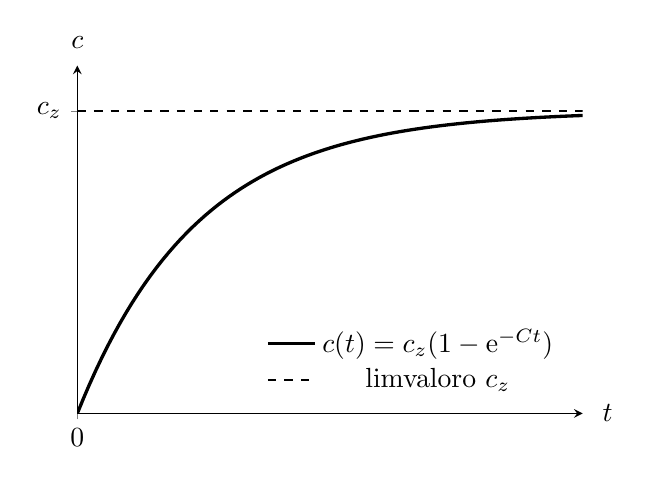
\begin{tikzpicture}
  % parametroj
  \pgfmathsetmacro{\cz}{10}
  \pgfmathsetmacro{\C}{1}

  \begin{axis}[
    width=8cm,
    height=6cm,
    axis lines=left,
    xlabel={$t$},
    ylabel={$c$},
    xlabel style={at={(ticklabel* cs:1.02)}, anchor=west},
    ylabel style={at={(ticklabel* cs:1.02)}, anchor=south, rotate=-90},
    xmin=0, xmax=4.2,
    ymin=0, ymax=11.5,
    xtick={0},
    ytick={\cz},
    yticklabels={$c_z$}, 
    grid=major,
    grid style={dashed, gray!30},
    samples=100, 
    domain=0:5,
    legend pos=south east,
    % --- stilo de legendo ---
    legend style={
      fill=none,   
      draw=none
    }    
  ]

    % funkcio: c(t) = c_z * (1 - exp(-C * t))
    \addplot[black, very thick] {\cz * (1 - exp(-\C * x))};
    \addlegendentry{$c(t) = c_z(1 - \mathrm{e}^{-Ct})$}

    % asimptoto ĉe c = c_z
    \addplot[black, dashed, thick] {\cz};
    \addlegendentry{limvaloro $c_z$}

  \end{axis}
\end{tikzpicture}
\end{document}